
En traitement du signal, la phase d'un signal est intrinsèquement liée à la notion de fréquence instantanée, qui joue un rôle important en analyse temps-fréquence. 
C'est donc de ce point que commencera notre discussion pour introduire la phase géométrique.
Pour cela, seront rapidement introduites quelques notions et résultats d'analyse temps-fréquence dans le cas univarié (sec. \ref{subsec:ana_temp-freq}). Suite à quoi, une notion de phase instantanée sera proposée dans le cas multivarié (sec. \ref{subsec:intro_phased}), ce qui permettra, enfin, de mettre en évidence la phase géométrique (sec. \ref{subsec:intro_phaseg}).
\\

Dans une seconde partie, seront introduits les signaux bivariés dits AM-FM-PM, dont la phase géométrique sera calculée explicitement (sec. \ref{subsec:AM-FM-PM}), ce qui permettra de mettre en évidence certaines de ses propriétés (sec. \ref{subsec:phase_g2Poincare}). Dans une dernière section, sera présenté une généralisation des signaux AM-FM-PM au-delà du cas bivarié (sec. \ref{subsec:aller_plus_loin}), ce qui mènera au formalisme de la \cref{part:phase_geo} suivante.
\\




\section{Introduction de la phase géométrique} \label{sec:intro_phaseg}

\subsection{Un peu d'analyse temps-fréquence} \label{subsec:ana_temp-freq}

En traitement du signal, l'analyse fréquentielle par la transformée de Fourier est un incontournable. 
Seulement, cette transformation fait perdre toute notion temporelle : si l'étude du spectre du signal permet de dire quelles fréquences apparaissent dans le signal, elle ne permet pas de dire à quel(s) moment(s). 
C'est en réponse à cela, entre autres, que fut développée l'analyse temps-fréquence et, à cette fin, sont définis les paramètres instantanées d'un signal :\par

\begin{definition}[Paramètres instantanés] \label{def:param_instant}
	Soit $x$ un signal complexe écrit sous forme exponentielle :
	\begin{align}
		x\ &:\ \begin{aligned}\R\ &\lr\qquad \C \\
			t\ &\longmapsto\ a(t)e^{\i \phi(t)}
		\end{aligned}  &  \text{où }\quad a(t)\in\R^+\quad &\text{et}\quad \phi(t)\in\R
	\end{align}
	$a$ est appelé \emph{amplitude instantanée} du signal, la dérivée $\nicefrac{\phi'}{2\pi}$ sa \emph{fréquence instantanée} et sa \emph{phase instantanée} est définie --- modulo un choix de phase initiale --- par :
	\begin{equation} \label{eq:phasei}
		\phasei(x,t_0,t) = \phi(t) - \phi(t_0)
	\end{equation}
\end{definition}
\skipl 

Pour les signaux réels, ces notions sont moins évidentes à définir puisqu'elles demandent d'écrire les signaux sous la forme :
\[x(t) = a(t) \cos\phi(t)\]
\\
Auquel cas, le choix de la paire $(a,\phi)$ n'est pas unique. Il existe tout de même un ``bon'' choix dans le cas des signaux AM-FM :
\begin{definition}[Signal AM-FM]
	Un signal réel de la forme :
	\begin{align}
		x\ &:\ \begin{aligned}\R\ &\lr\qquad \R \\
			t\ &\longmapsto\ a(t) \cos\phi(t)
		\end{aligned}  &  \text{où }\quad a(t)\in\R^+\quad
	\end{align}
	est dit \emph{AM-FM} (\emph{amplitude and frequency modulated}) si $a$ et $\cos\phi$ admettent une transformée de Fourier et si, de plus, la première a un spectre concentré sur les basses fréquences, la seconde concentré sur les hautes fréquences et que les deux ne se chevauchent pas.
	Formellement, ces conditions demandent qu'il existe $\lambda\in\R^+$ tel que :
	\begin{equation}\label{eq:condi_AM-FM}
		\supp \Fou{a} \subset [-\lambda, \lambda],\quad \supp \Fou{\cos\phi} \subset \R\setminus[-\lambda,\lambda]
	\end{equation}
	\\
	Dans ce cas, $a$ et $\phi$ donnent lieu au même vocabulaire que pour le cas complexe (\cref{def:param_instant}).
\end{definition}
\skipl
\\
Ces conditions sont liées au théorème de Bedrosian, et plus de détails se trouvent dans l'annexe \ref{ann:complement_t-f}. Pour le dire rapidement, exiger que toutes les hautes fréquences de $x$ se trouvent dans la phase traduit l'idée que l'amplitude doit moduler la phase, et non l'inverse. Pour que ce soit possible, il est donc nécessaire que les variations de l'amplitude reste marginale par rapport à celle de la phase. Contrainte qui se traduit bien la condition \eqref{eq:condi_AM-FM} sur la distribution des spectres de $a$ et $\cos\phi$.
\\
Sous ces conditions, $x$ peut être vu comme le signal complexe $\SA{x}$ tel que :
\begin{equation}
	\forall t\in\R,\qquad \SA{x}(t) = a(t) e^{\i \phi(t)}= a(t)\cos\phi(t) + \i a(t)\sin\phi(t)
\end{equation}
\\
Ce signal $\SA{x}$ est appelé \emph{transformée en signal analytique de} $x$ et a, par construction, les mêmes paramètres instantanées que $x$.
Là encore, le lecteur est renvoyé vers l'annexe \ref{ann:complement_t-f} pour plus de détails ou bien dans le livre de Cohen \cite{cohen_time_1995}.
\\

L'intérêt d'introduire toutes ces notions est que les signaux multivariés --- même complexes --- souffrent du même problème que les signaux réels. 
En effet, en écrivant un signal $\x$ sous la forme :
\[\forall t\in\R,\qquad 
\x(t) = \begin{pmatrix} A_1(t)e^{\i \phi_1(t)} \\ A_2(t)e^{\i \phi_2(t)} \\ \vdots \\ A_n(t)e^{\i \phi_n(t)}
\end{pmatrix}\]
\\
le fait que $\x$ soit à valeur dans $\C^n$ impose un choix naturel d'amplitude instantanée : sa norme. Pour ce qui est de la phase instantanée, en revanche, n'importe quel choix de $\phi$ convient \apriori. En écrivant :
\[\forall t\in\R,\qquad 
\x(t) = \begin{pmatrix} A_1(t)e^{\i \phi_1(t)} \\ A_2(t)e^{\i \phi_2(t)} \\ \vdots \\ A_n(t)e^{\i \phi_n(t)} \end{pmatrix}
= a(t)e^{\i \phi(t)}\begin{pmatrix} a_1(t)e^{\i \psi_1(t)} \\ a_2(t)e^{\i \psi_2(t)} \\ \vdots \\ a_n(t)e^{\i \psi_n(t)} \end{pmatrix}
\qquad\text{ avec }\qquad 
\left\{ \begin{aligned}
	& a(t) = \| \x(t) \|_2 \\
	& \sum_{i=1}^n {a_i}^2 = 1 \\
	& \phi_i = \phi + \psi_i \end{aligned}\right.\]
\\
il suffit que les $\psi_i$ soient ajustés pour assurer que $\ \phi_i = \phi + \psi_i$.
\\
\begin{remarque}
	Si $a$ et $\phi$ correspondent respectivement à une amplitude et une phase, le vecteur restant $\big( a_ie^{\i \phi_i} \big)_{1\leq i\leq n}$ correspond à un état de polarisation, sur lequel nous reviendrons dans la \cref{sec:AM-FM-PM} suivante.
\end{remarque}
\skipl




\subsection{Phase et fréquence instantanée de signaux multivariés} \label{subsec:intro_phased}

On se propose ici de définir la phase instantanée comme suit :
\begin{definition}[Phase dynamique/instantanée] \label{def:phase_d}
	La \emph{phase instantanée} ou \emph{dynamique} (à l'instant $t$ partant de $t_0$) d'un signal multivarié $\x = a\big(a_ie^{\i \phi_i}\big)_{1\leq i\leq n} \in \conti[1]{\R}{\C^n}$, est donnée par la formule :
	\begin{equation} \label{eq:phase_d}
		\forall t_0, t\in\R, \quad \phased[\x](t_0,t) \defeq \int_{t_0}^t \frac{\Im m \big\langle \dot{\x}(s) , \x(s) \big\rangle}{\|\x(s)\|^2} ds =\sum_{i=1}^n \int_{t_0}^t a_i(s)^2 \phi_i'(s)ds
	\end{equation}
	\\
	On s'autorisera à omettre les paramètres de $\phased$ lorsque cela ne prête pas à confusion.
\end{definition}
\skipl

Cette définition est motivée par deux arguments :



\subsubsection*{\textbullet\ Argument variationnel}

Le premier, fortement inspiré par les travaux de Lilly \& Olhede  \cite{lilly_analysis_2012}, consiste à généraliser la condition \eqref{eq:condi_AM-FM} de séparation hautes/basses fréquences sur les signaux AM-FM.
Pour cela, on commence par faire apparaître une phase $\phi$ --- pour l'instant inconnue --- en écrivant $\x$ sous la forme :
\[\forall t\in\R,\qquad \x(t) = e^{\i \phi(t)} e^{-\i \phi(t)} \x(t) \defeq e^{\i \phi(t)} \bf{y}_\phi(t)\]
\\
Si $\phi$ est bien choisie, alors $\bf{y}_\phi$ ne devrait contenir que les informations associées à l'amplitude et à la polarisation de $\x$. Or, conformément à la condition \eqref{eq:condi_AM-FM}, la phase doit contenir les hautes fréquences du signal et, inversement, les basses fréquences doivent se trouver dans le reste. 
\\
La fréquence donnant, pour le dire vite, la vitesse d'ondulation, la contrainte sur $\x$ va être de limiter les variations de  $\bf{y}_\phi$. Concrètement, $\phi$ doit être choisie de sorte à minimiser la dérivée $\dot{\bf{y}}_\phi$ :
\[\forall t\in\R,\qquad \phi(t) = \argmin{\theta(t)}{\big\|\dot{\bf{y}}_\theta(t)\big\|_2}^2 = \argmin{\theta(t)}{\Big\|e^{-\i \theta(t)}\big(\dot{\x}(t) - i\theta'(t) \x(t)\big) \Big\|_2}^2 = \argmin{\theta(t)}{\big\|\dot{\x}(t) - i\theta'(t)\x(t)\big\|_2}^2\]
\\
La contrainte ne dépendant que de la dérivée $\theta'$, on se ramène à :
\[\min_{\theta(t)}{\|\dot{\bf{y}_\theta}(t)\|_2}^2 = \min_{\theta'(t)}{\big\|\dot{\x}(t) - i\theta'(t) \x(t)\big\|_2}^2\]
\\
En rappelant que $\frac{d}{dx}{\big\|f(x)\big\|_2}^2 = 2\Re e\big\langle f(x), f'(x)\big\rangle$, il vient que l'unique minimum\footnote{\itshape
	L'extremum obtenu est l'unique minimum globale puisque $t\longmapsto \|at + b\|^2$ est strictement convexe pour $a\neq0$.}
est atteint par $\phi'(t)$ à condition que :
\begin{align*}
	\frac{d}{d\phi'}{\big\| \dot{\x} - i\phi' \x\big\|_2}^2 = 0 \quad \Llr\quad
	0 &= 2\Re e\left\langle  \dot{\x} - i\phi' \x ,  \frac{d}{d\phi'}\big(\dot{\x} - i\phi' \x\big)\right\rangle \\
	&= 2\Re e\big\langle  \dot{\x} - i\phi' \x ,  - i \x\big\rangle \\
	&= 2\Re e\Big(i\big\langle  \dot{\x} ,  \x\big\rangle\Big) + 2\phi'\Re e\big\langle   \x ,  \x\big\rangle\\
	&= -2\Im m\big\langle  \dot{\x} ,  \x\big\rangle + 2\phi'{\| \x\|_2}^2
\end{align*}
Ainsi $\displaystyle \ \phi' = \frac{\Im m\big\langle \dot{\x} ,  \x\big\rangle}{{\| \x\|_2}^2}\ $ et :
\begin{equation}\label{eq:phas_inst_v1}
	\phi(t) = \Im m\int_{t_0}^t \frac{\big\langle \dot{\x}(s) , \x(s) \big\rangle}{\|\x(s)\|^2} ds = \phased[\x](t_0,t)
\end{equation}
\skipl




\subsubsection*{\textbullet\ Arguments des moyennes}

Le second argument, cette fois inspiré de \cite{cano_mathematical_2022}, se base sur la notion de fréquence moyenne.
D'abord dans le cas d'un signal complexe univarié, sont définies les fonctions de densités d'énergie (resp. d'énergie spectrale) comme :
\begin{align}\label{eq:densi_dE}
	\densit\ &:\quad \begin{aligned}\R\ &\lr\quad \R^+ \\ t\ &\longmapsto\ \big|x(t)\big|^2 \end{aligned}  
	&
	\text{resp.}\qquad \densis\ &:\quad \begin{aligned}\R\ &\lr\quad \R^+ \\ \nu\ &\longmapsto\ \big|\fou{x}(\nu)\big|^2 \end{aligned}
\end{align}
\\
À partir de ces dernières est définie la fréquence moyenne de $x$ comme l'espérance $\esp[\densis]{\nu}$ de $\densis$\footnote{\itshape
	La notation avec l'espérance n'est pas complètement appropriée puisque $\densit$ n'est pas une densité de probabilité (non normalisée). Cela dit, on peut supposer sans perte de généralité que $\ \|\densit\|_2 = \|\densis\|_2 = 1\ $ et, dans tous les cas, l'interprétation en terme de moyenne tient toujours.
}. Cette fréquence moyenne est liée à la fréquence instantanée par la formule\footnote{\itshape
	Cette formule de généralise à tous les moments de $\densis$ et existe également pour les moments de $\densit$, voir \cite[sec. 1.4]{cohen_time_1995} pour une démonstration.}
:
\begin{equation}\label{eq:esp_freq}
	\esp[\densis]{\nu} = \frac{1}{2\pi}\int_\R \phi'(t)\densit(t)dt = \esp[\densit]{\frac{1}{2\pi} \phi'}
\end{equation}
\\
Dans le cas d'un signal $\x=(x_i)_{1\leq i\leq n}$ multivarié, les densités d'énergies se définissent comme :
\begin{align*}%\label{eq:densi_dEi}
	\densit_i\ &:\quad \begin{aligned}\R\ &\lr\quad \R^+ \\ t\ &\longmapsto\ \big|x_i(t)\big|^2 = a(t)^2 a_i(t)^2 \end{aligned}  
	&
	\densis_i\ &:\quad \begin{aligned}\R\ &\lr\quad \R^+ \\ \nu\ &\longmapsto\ \big|\fou{x}_i(\nu)\big|^2 \end{aligned} \\ \\
	%\label{eq:densi_dE-mv}
	\densit\ &:\quad \begin{aligned}\R\ &\lr\quad \R^+ \\ t\ &\longmapsto\ \big\|\x(t)\big\|^2 = \sum_{i=1}^n \densit_i(t) \end{aligned}  
	&
	\densis\ &:\quad \begin{aligned}\R\ &\lr\quad \R^+ \\ \nu\ &\longmapsto\ \big\|\fou{\x}(\nu)\big\|^2 = \sum_{i=1}^n \densis_i(t) \end{aligned}	
\end{align*}
Le second argument consiste alors à dire que l'égalité des moyennes $\eqref{eq:esp_freq}$ doit rester valable dans le cas multivarié. Cela assure, à minima, que la fréquence instantanée de $\x$, $\nicefrac{1}{2\pi}\phi'$, à pour moyenne $\esp[\densis]{\nu}$.
\\

En appliquant la formule \eqref{eq:esp_freq} aux $\densis_i$, et en notant toujours $\x = a\big(a_1e^{\i \phi_1}, \cdots, a_ne^{\i \phi_n}\big)$, on obtient :
\begin{align*}
	\esp[\densis]{\nu} = \int_\R \nu\densis(\nu)d\nu &= \int_\R \nu\sum_{i=1}^n \densis_i(\nu) d\nu \\
	&= \sum_{i=1}^n\esp[\densis_i]{\nu} \\
	&= \sum_{i=1}^n\frac{1}{2\pi}\int_\R \phi_i'(t)\densit_i(t)dt \\
	&= \frac{1}{2\pi}\int_\R a(t)^2\sum_{i=1}^n\phi_i'(t)a_i(t)^2 dt \\
	&= \esp[\densit]{\frac{1}{2\pi}\sum_{i=1}^n \phi_i'{a_i}^2}
\end{align*}
\\
Ce qui mène à poser $\displaystyle \ \sum_{i=1}^n \phi_i'(t){a_i}^2(t)\ $ pour la fréquence instantanée, avec la phase associée :
\begin{equation}\label{eq:phas_inst_v2}
	\phi = \int_{t_0}^t \sum_{i=1}^n \phi_i'(s){a_i}(s)^2ds 
	= \sum_{i=1}^n \int_{t_0}^t \phi_i'(s){a_i}(s)^2ds 
	%= \sum_{i=1}^n \esp[\nicefrac{\densit_i}{\densit}]{\phi_i'}
\end{equation}
\\

Formule qui concorde bien avec celle de la phase dynamique une fois explicitée :
\begin{align*}
	\Im m\frac{\big\langle \dot{\x}(t) , \x(t) \big\rangle}{\|\x(t)\|^2} &= \Im m\left( \frac{1}{a(t)^2} \sum_{i=1}^n \Big( \big(aa_i\big)'(t) +a(t)a_i(t)i\phi_i'(t)\Big)e^{\i \phi_i(t)}\congu{a(t)a_i(t)e^{\i \phi_i(t)}} \right) \\
	&=\frac{1}{a(t)^2}  \Im m\left( \sum_{i=1}^n a(t)a_i(t)\big(aa_i\big)'(t) +\i a(t)^2a_i(t)^2\phi_i'(t) \right) \\
	&= \frac{1}{a(t)^2} \sum_{i=1}^n a(t)^2a_i(t)^2 \phi_i'(t) \\
	&= \sum_{i=1}^n a_i(t)^2 \phi_i'(t)
\end{align*}
D'où
\[\Im m\int_{t_0}^t \frac{\big\langle \dot{\x}(s) , \x(s) \big\rangle}{\|\x(s)\|^2} ds = \int_{t_0}^t \sum_{i=1}^n a_i(s)^2 \phi_i'(s) = \sum_{i=1}^n \int_{t_0}^t a_i(s)^2 \phi_i'(s)ds\]
\skipl



\subsection{Apparition de la phase géométrique}\label{subsec:intro_phaseg}

Cela étant dit, il existe une autre façon, plus simple, d'obtenir la phase d'un signal. D'abord, dans le cas univarié, la phase instantanée de $x=ae^{\i \phi}$ peut être réécrite comme :
\[\phi(t)-\phi(t_0)  = \arg\left( x(t) \congu{x(t_0)} \right)\]
\\
Formule qui se généralise en cas multivarié par ce qui sera appelé la \emph{phase totale} du signal :
\begin{equation}\label{eq:phase_t}
	\phaset(\x, t_0, t) \defeq \arg\big\langle \x(t), \x(t_0)\big\rangle
\end{equation}
\\
D'un point de vu géométrique, il est bien connu que le produit scalaire entre deux vecteurs réels $u,v\in\R^n$ est lié à l'angle $\angle(u,v)$ entre ces derniers par la formule :
\[\langle u,v\rangle_\R = \|u\|^2 \|v\|^2 \cos \angle(u,v)\]
\\
Pour le produit hermitien, cet angle ce retrouve dans l'argument, de sorte que si $u$ et $v$ sont complexes :
\[\langle u,v\rangle_\C = \|u\|^2 \|v\|^2 e^{\i  \angle(u,v)}\]
\\
En ce sens, la phase totale calcule explicitement l'angle entre $\x(t_0)$ et $\x(t)$ et il est montré, dans le cas univarié, qu'elle est égale à la phase dynamique. En effet, pour $\x = ae^{\i \phi}$ :
\begin{align*}
	\phased[\x] = \Im m\int_{t_0}^t \frac{\big\langle \dot{\x}(s) , \x(s) \big\rangle}{\|\x(s)\|^2} ds &= \Im m \int_{t_0}^t \frac{\big(a'(s) + \i a(s)\phi'(s) \big) e^{\i \phi(s)} \congu{a(s) e^{\i \phi(s)}}}{a^2(s)} ds \\
	&= \int_{t_0}^t \frac{a^2(s)\phi'(s))}{a^2(s)} ds \\
	&= \phi(t) - \phi(t_0) = \phaset(\x)
\end{align*}
\skipl

Dans le cas multivarié, en revanche, c'est une autre histoire. En notant cette fois le signal \\
$\x = ae^{\i \phased} \big( a_ie^{\i \psi_i} \big)_{1\leq i\leq n}$, la phase totale se réécrit :
\begin{equation}\label{eq:diff_phases_t/d}
	\begin{aligned}
		\phaset(\x,t_0, t) &= \arg \left(a(t)a(t_0) e^{\i \big(\phased(t) - \phased(t_0)\big)}\sum_{i=1}^n a_i(t)a_i(t_0)e^{\i (\psi_i(t)-\psi_i(t_0))} \right) \\
		&= \phased(t) + \arg \left(\sum_{i=1}^n a_i(t)a_i(t_0)e^{\i (\psi_i(t)-\psi_i(t_0))} \right)  \qquad\qquad\qquad\qquad \text{car } \phased(t_0,t_0) = 0
		%\\ &= \phased + \arctan \left( \frac{\sum_i a_i(t)a_i(t_0)\sin\big( \psi_i(t)-\psi_i(t_0)\big)}{\sum_i a_i(t)a_i(t_0)\cos\big( \psi_i(t)-\psi_i(t_0)\big)}  \right)
	\end{aligned}
\end{equation}
\\
Apparaît alors un terme de déviation de la phase dynamique par rapport à la phase totale, appelé (surprise) phase géométrique et noté :
\begin{equation}\label{eq:phase_g}
	\phaseg(\x,t_0,t) \defeq \phaset(\x, t_0,t) - \phased[\x](t_0,t)
\end{equation}
Cette déviation s'observe expérimentalement, comme le montre la \Cref{fig:calc_diff_phases} ci-dessous.
\\
\begin{figure}[h]
	
\includegraphics[width=0.6\textwidth]{fig/placeholder}
	\caption[Déviation de la phase dynamique d'un signal bivarié par rapport à sa phase totale]{Sur le graphe de gauche, le signal $\x$ est à valeurs dans $\R^2$. Dans celui de droite, le calcul des phases dynamique et totale de $\SA{\x}$,  ainsi que de leur différence. %Résultat tiré des simulation de Le Bihan \etal~\cite{le_bihan_modephysiques_2023}
	}
	\label{fig:calc_diff_phases}
\end{figure}
\\

Comme mentionné en introduction, un résultat bien connu en physique \cite{bohm_geometric_2003,mukunda_quantum_1993,chruscinski_geometric_2004} est que cette troisième phase est invariante par transformation de jauge et par reparamétrisation.
Dans notre contexte, cela signifie d'une part que si $\x$ et $\Tilde{\x}$ sont deux signaux multivariés complexes tels que $\ \Tilde{\x} = e^{\i \alpha}\x$, avec $\alpha$ une \underline{fonction} dérivable du temps, alors :
\begin{align*}
	\phaseg(\Tilde{\x}) &= \phaset(\Tilde{\x}) - \phased(\Tilde{\x})  = \phaset(\x) - \phased(\x) = \phaseg(\x)\\
	%&= \arg\big\langle \Tilde{\x}(t), \Tilde{\x}(t_0)\big\rangle - \Im m\int_{t_0}^t \frac{\big\langle \dot{\Tilde{\x}}(s) , \Tilde{\x}(s) \big\rangle}{\|\Tilde{\x}(s)\|^2} ds \\
	%&= \arg\big\langle e^{\i \alpha(t)}\x(t), e^{\i \alpha(t_0)}\x(t_0)\big\rangle - \Im m\int_{t_0}^t \frac{\big\langle \dot{e^{\i \alpha(s)}\x}(s) , e^{\i \alpha(s)}\x(s) \big\rangle}{\|e^{\i \alpha(s)}\x(s)\|^2} ds 
\end{align*}
Et d'autre part que, pour tout difféomorphisme $\gamma$ de $\R$ tel que :
\begin{align*}
	\x\circ\gamma(s_0)&=t_0  &  \x \circ\gamma(s) = t
\end{align*}
on a :
\[\phaseg(\x \circ \gamma, s_0, s) = \phaseg(\x, t_0, t)\]
\skipl


D'un point de vue signal, cette invariance par transformation de jauge indique que $\phaseg$ est lié à une notion de polarisation du signal, chose que nous allons à présent mettre en évidence à travers un exemple.
\\



\section{Première cas d'étude : les signaux AM-FM-PM} \label{sec:AM-FM-PM}

Pour une première étude de la phase géométrique du signal, Le Bihan, Flamant \& Amblard se sont penchés sur un cas particulier de signal bivarié \cite{flamant_timefrequency_2019,le_bihan_modephysiques_2023, le_bihan_geometric_2024}. Ces signaux, AM-FM-PM, sont présentés dans une première partie avec le calcul explicite de leur phases --- totale, dynamique et géométrique --- puis sera introduite la sphère de Poincaré, sur laquelle $\phaseg$ pourra être interprétée.
Cela mènera à proposer un modèle pour décrire les signaux multivariés complexes, modèle très largement inspiré par ce qui a déjà été fait dans l'étude de la phase géométrique.
\\



\subsection{Définitions et calcul des phases} \label{subsec:AM-FM-PM}

Ces signaux AM-FM-PM viennent généraliser les signaux AM-FM univariés en tenant compte de l'état de polarisation permis par l'accès à une seconde dimension. 
En quelques mots, dans le cas le plus simple, un signal bivarié à valeurs \emph{réelles} $s$ décrit une ellipse au cours du temps. 
On parle de polarisation elliptique et $s$ s'écrit :
\[s(t) = a \begin{pmatrix} \cos\theta & -\sin\theta \\ \sin\theta  &  \cos\theta \end{pmatrix} \begin{pmatrix} \cos\chi \cos\varphi(t) \\ \sin\chi \sin\varphi(t) \end{pmatrix}  \qquad \text{ où }\quad  a\in\R^+,\ \theta \in \left]-\frac{\pi}{2}, \frac{\pi}{2}\right],\ \chi \in \left[-\frac{\pi}{4}, \frac{\pi}{4}\right] \]
\\
Les paramètres $a$ et $\chi$ caractérisent respectivement la taille et l'excentricité de l'ellipse, $\theta$ son orientation dans le plan et $\varphi(t)$ précise où se trouve $s$ à l'instant $t$ sur cette ellipse. Le signe de $\chi$ donne également le sens de rotation de $\varphi$ sur l'ellipse (trigonométrique ou anti-trigonométrique), le tout est représenté sur la \Cref{fig:ellipse2polar} ci-dessous :
\begin{figure}[H]
	%
\includegraphics[width=0.45\textwidth]{fig/placeholder}
	\makeatletter % fonction pour increasing width !
	\pgfkeys{/pgf/decoration/.cd,
		start color/.store in =\startcolor,
		end color/.store in   =\endcolor
	}
	
	\pgfdeclaredecoration{width and color change}{initial}{
		\state{initial}[width=0pt, next state=line, persistent precomputation={%
			\pgfmathdivide{50}{\pgfdecoratedpathlength}%
			\let\increment=\pgfmathresult%
			\def\x{0}%
		}]{}
		\state{line}[width=.5pt,   persistent postcomputation={%
			\pgfmathadd@{\x}{\increment}%
			\let\x=\pgfmathresult%
		}]{%
			\pgfsetlinewidth{\x/80*0.001pt+\pgflinewidth}%
			\pgfsetarrows{-}%
			\pgfpathmoveto{\pgfpointorigin}%
			\pgfpathlineto{\pgfqpoint{.75pt}{0pt}}%
			\pgfsetstrokecolor{\endcolor!\x!\startcolor}%
			\pgfusepath{stroke}%
		}
		\state{final}{%
			\pgfsetlinewidth{\pgflinewidth}%
			\pgfpathmoveto{\pgfpointorigin}%
			\color{\endcolor!\x!\startcolor}%
			\pgfusepath{stroke}% 
		}
	}
\makeatother


\begin{tikzpicture}[scale=1]
	%\draw[black, opacity=0.3] (-4.5,-4.5) grid (4.5,4.5);
	\draw[opacity=1, -Stealth] (0,-4) -- (0,4);
	\draw[opacity=1, -Stealth] (-4,0) -- (4,0);
	
	\coordinate (o) at (0,0);
	\coordinate (i) at (4,0);
	\coordinate (j) at (0,4);
	\coordinate (theta) at (40:4);
	
	
	%axis de l'ellipse
	\draw[thick, opacity=0.9, rotate = 40] (-4,0) -- (o) node[midway, below, rotate=40]{$a\cos\chi$} -- (4,0);
	\draw[thick, opacity=0.9, rotate = 40] (0,-3) -- (o) -- (0,3) node[midway, above, rotate=-50]{$a\sin\chi$};
	
	% paramètres
		
		%theta
	\draw[opacity=0.9, -stealth] (2, 0) arc [start angle=0, end angle =40, radius = 2] node[midway, right]{$\theta$};
		
		%chi
	\draw[opacity=0.8, -stealth, rotate = 40] (-2,0) arc [start angle=0, end angle =37, radius = 2] node[midway, above right]{$\chi$};
	
	\draw[opacity=0.8, rotate = 40] (-4,0) -- (0,3);
		
		%varphi
	\draw[color=blue, opacity=0.8, -stealth, rotate = 40] (0.75,0) arc [start angle=0, end angle =60, radius = 0.75] node[midway, above right]{$\varphi$};
	
	\draw[color=blue, opacity=0.8, rotate = 40] (o) -- (60:3.18);
	
	\fill[blue] (100:3.18) circle (0.05);
	
	% ellipse
	\draw[line width=0.5pt, rotate=40, decoration={width and color change, start color=black, end color=blue}, decorate] (60:3.18) arc [start angle=66.65, end angle =426.65, x radius = 4, y radius = 3];
	
\end{tikzpicture}
	\caption[\DONE Ellipse de polarisation d'un signal bivarié réel]{Ellipse de polarisation du signal $s$ sur laquelle sont représentés ses paramètres $a,\varphi,\theta$ et $\chi$.}
	\label{fig:ellipse2polar}
\end{figure}
\skipl \\
En autorisant les paramètres de polarisation à varier au cours du temps et après une transformation en signal analytique, mentionnée dans la \cref{subsec:ana_temp-freq}, on obtient la définition suivante :
\\
\begin{definition}[Signal AM-FM-PM] \label{def:AM-FM-PM}
	Un signal bivarié complexe $\x$ \emph{AM-FM-PM} (\emph{amplitude, frequency and polarization modulated}) est caractérisé par quatre paramètres $a,\varphi,\theta$ et $\chi$, respectivement à valeurs dans $\R^+$, $\R$, $]-\frac{\pi}{2}, \frac{\pi}{2}]$ et $[-\frac{\pi}{4}, \frac{\pi}{4}]$, vérifiant :
	\begin{align}\label{eq:condi_AM-FM-PM}
		\big| \varphi'(t) \big| &\gg \big| \theta'(t) \big| ,\ \big| \chi'(t) \big| ,\ \left| \frac{a'(t)}{a(t)}\right|  &  \left| \frac{\varphi'(t)}{\varphi(t)}\right| \gg 1
	\end{align}
	Auquel cas, $\x$ prend la forme, $\forall t\in\R$ :
	\begin{equation}\label{eq:AM-FM-PM}
		\x(t) = a(t)e^{\i \varphi(t)} R_{\theta(t)} \begin{pmatrix} \cos\chi(t) \\ -\i\sin\chi(t) \end{pmatrix} 
		= a(t)e^{\i \varphi(t)} \begin{pmatrix} \cos\theta(t) \cos\chi(t) + \i\sin\theta(t) \sin\chi(t) \\ \sin\theta(t) \cos\chi(t) - \i\cos\theta(t) \sin\chi(t) \end{pmatrix}
	\end{equation}
	où $R_{\theta(t)}$ est la matrice de rotation d'angle $\theta(t)$. Voir \cite[ann. 4.B]{flamant_approche_2018} pour une construction plus détaillée.
\end{definition}
\skipl

Jusqu'à présent, la phase géométrique n'a été étudiée que dans le cadre complexe et pour cette raison, il est nécessaire de passer par la transformée en signal analytique (\cf~annexe \cref{ann:complement_t-f}).
La transformation du signal à valeurs réelles en un signal à valeurs complexes est nécessaire pour étudier la phase géométrique car c'est uniquement dans le cadre complexe qu'elle a été étudiée jusqu'à présent. 
Et, comme pour les signaux AM-FM, les hypothèses sur $a,\varphi,\theta,\chi$ assure que les paramètres restent interprétables suivant la \Cref{fig:ellipse2polar} précédente.
\\

Les trois phases de tels signaux sont données par la \cref{prop:phases_2var} suivante :
\begin{proposition}[phases de signal AM--FM--PM]\label{prop:phases_2var}
	Les trois phases d'un signal bivarié AM--FM--PM $\x$ 	de paramètres $(a,\varphi,\theta,\chi)$ sont données par les formules :
	\begin{equation}\label{eq:phaset_2var}
		\begin{aligned}
			\phaset(\x,t_0,t) &= \varphi(t)-\varphi(t_0) + \arg\Big(\cos\Delta\theta \cos\Delta\chi + \i\sin\Delta\theta \sin\big(\chi(t_0)+\chi(t)\big)\Big)
		\end{aligned}
	\end{equation}
	\begin{equation}\label{eq:phased_2var}
		\phased[\x](t_0,t) = \varphi(t) -\varphi(t_0) + \int_{t_0}^t\theta'(s) \sin2\chi(s) ds
	\end{equation}
	\begin{equation}\label{eq:phaseg_2var}
		\begin{aligned}
			\phaseg(\x,t_0,t) &= \phaset(\x,t_0,t) - \phased(\x,t_0,t) \\
			&= \arg\Big(\cos\Delta\theta \cos\Delta\chi + \i\sin\Delta\theta \sin\big(\chi(t_0)+\chi(t)\big)\Big) - \int_{t_0}^t\theta'(s) \sin2\chi(s) ds
		\end{aligned}
	\end{equation}
	\\
	où $\ \Delta y = y(t) - y(t_0)\ $ pour $\ y = \chi, \theta$. La démonstration se trouve en annexe \ref{ann:demo_phases_2var}.
\end{proposition}
\skipl

\begin{figure}[h]
	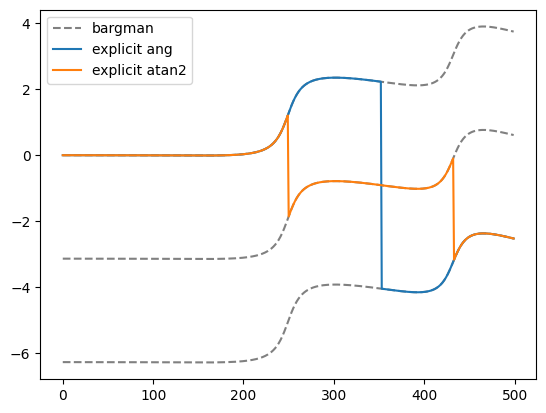
\includegraphics[width = 0.6\textwidth]{fig/premier_resultat}
	\caption[Evolution de la phase géométrique d'un signal AM-FM-PM]{Evolution de la phase géométrique d'un signal AM-FM-PM généré. En gris la phase géométrique du signal calculé via l'invariant de Bargmann (\cf~\cref{part:app&gene}), fonction reprise des travaux de Le Bihan \etal \cite{le_bihan_modephysiques_2023,le_bihan_geometric_2024}. Les deux autres sont calculées avec la formule \cref{eq:phaseg_2var}, en bleu en utilisant de l'argument pour la phase totale et en orange en utilisant atan2. Les saut présents sur la figure sont dû au fait que la phase géométrique soit définie modulo $2\pi$.}
\end{figure}

Deux remarques sur ces formules. 
La première est que la phase géométrique ne dépend que des paramètres de polarisations $\theta$ et $\chi$, ce qui reflète son invariance par transformation de jauge.
La seconde, nettement plus troublante, est que $\varphi$ ne s'interprète ni comme phase totale ni comme phase dynamique, un point qui sera expliqué dans la \cref{part:phase_geo}.
\\
Un moyen d'avoir cette interprétation est de supposer qu'à l'instant $t$, $\x $ retrouve la même polarisation instantanée qu'à l'instant $t_0$, auquel cas :
\begin{equation}\label{eq:phases_p-cyc_2var}
	\begin{aligned}
		\big( \chi(t), \theta(t) \big) = \big( \chi(t_0), \theta(t_0) \big)\quad 
		&\Lr\quad \phaset(\x ) = \varphi(t) - \varphi(t) \\
		&\Lr\quad \phaseg(\x ) = -\int_{t_0}^t \theta'(s) \sin 2\chi(s) ds
	\end{aligned}
\end{equation}
\skipl

Même dans ce cas, il est utile de d'avoir une représentation de $\x $ qui soit indépendante de sa phase pour interpréter cette formule \eqref{eq:phases_p-cyc_2var}.
\\



\subsection{Interprétation sur la sphère de Poincaré}\label{subsec:phase_g2Poincare}

Dans l'étude de la phase géométrique, il est standard de s'intéresser à la matrice de covariance\footnote{\itshape
	Il est plus commun en physique de conjuger à droite, mais la conjugaison à gauche simplifie l'interprétation de $\rho$ dans la \Cref{fig:sphere2poincare}. Cela est également plus cohérent avec notre définition du produit hermitien qui utilise la convention $\ \langle x, y\rangle = \transp{x}\congu{y}$.
} :
\begin{equation} \label{eq:proj2x_2var}
	\forall t\in\R,\quad \rho_{\x}(t) = \frac{1}{\|\x(t) \|^2} \congu{\x(t) }\, \transp{\x}(t)
\end{equation}
\\
Outre son utilité en traitement du signal, elle présente l'avantage d'être invariante par transformation de jauge (\ie~ $\rho_{e^{\i \alpha}\x} = \rho_{\x}$).
Aussi ces matrices sont connues \cite{brosseau} pour avoir pour base les matrices de Pauli $\sigma_i$, ce qui, dans le cas des signaux AM-FM-PM, donne \cite{le_bihan_geometric_2024} :
\begin{equation} \label{eq:decompo_pauli}
	\rho_{\x} = \frac{1}{2}\Big( \Id + \sin(2\theta) \cos(2\chi) \sigma_1 + \sin (2\chi) \sigma_2 + \cos(2\theta) \cos(2\chi) \sigma_3 \Big)
\end{equation}


\begin{wrapfigure}{r}{0.4\textwidth}
	%
\includegraphics[width=0.9\textwidth]{fig/placeholder}
	\begin{tikzpicture}[scale=0.8]
	%\draw[black, opacity=0.1] (-4.5,-4.5) grid (4.5,4.5);
	\draw[-Stealth] (-2.5,0) -- (4.5,0) node[below]{$\sigma_1$};
	\draw[-Stealth] (0,-4.5) -- (0,4.5) node[right]{$\sigma_2$};
	\draw[-Stealth] (2.5,1.2) -- (-2.5,-1.2)  node[below right]{$\sigma_3$};
	
	\coordinate (o) at (0,0);
	\coordinate (i) at (4,0);
	\coordinate (j) at (0,4);
	
	\coordinate (u) at (2.1,2.14);
	\coordinate (p) at (2.1, -0.5);
	\coordinate (v) at (3.4,0.5);
	
	% cercles
	\draw[thick] (4,0) arc [start angle=0, end angle =-140, radius = 4];
	\draw[thick] (4,0) arc [start angle=0, end angle =100, radius = 4];
	
	\draw[thick, dashed] (4,0) arc [start angle=0, end angle =100, radius = 4, y radius = 1];
	\draw[thick] (4,0) arc [start angle=0, end angle =-125, x radius = 4, y radius = 1];
	
	% droites
	\draw[-stealth,thick, blue] (0,0) -- (u) node[above right] {$\rho$};
	\draw[dashed, blue] (u) -- (p);
	\draw[dashed, blue] (0,0) -- (p);
	
	%arc au point
	\draw[gray, dashed] (3.1,2.5) arc [start angle=0, end angle =105, radius = 3.1, y radius = 0.5];
	\draw[gray] (3.1,2.5) arc [start angle=0, end angle =-120, x radius = 3.1, y radius = 0.5];
	
	\draw[violet, -stealth] (-0.4, -0.2) arc [start angle=-120, end angle =-40, x radius = 0.9, y radius = 0.225] node[midway, below] {\scriptsize$2\theta$};    
	\draw[violet, -stealth] (0,0.7) arc [start angle=90, end angle =20, x radius = 0.4, y radius = 0.5];
	\draw[violet] (0.25, 0.8) node{\scriptsize$2\chi$};
\end{tikzpicture}
	\caption[\DONE Projection sur la sphère de Poincaré]{Représentation de $\rho_{\x}$ sur la sphère de Poincaré en fonction des paramètres $\theta$ et $\chi$.}
	\label{fig:sphere2poincare}
\end{wrapfigure}

\par \noindent
où les $\sigma_i$ s'écrivent :
\begin{align*}
	\sigma_1 &= \begin{pmatrix} 0 & 1 \\ 1 &  0 \end{pmatrix}  &
	\sigma_2 &= \begin{pmatrix} 0 & -i \\  i &  0 \end{pmatrix}  &
	\sigma_3 &= \begin{pmatrix} 1 & 0 \\ 0 & -1 \end{pmatrix}
\end{align*}
\skipl

Dans cette décomposition, la composante en $\Id$ est indépendante de $\x$ et peut donc être ignorée (idem pour le facteur $\nicefrac{1}{2}$). Cela ne laisse qu'un vecteur (normé) de dimension 3 dont $2\theta$ et $2\chi$ correspondent aux coordonnées sphériques conformément à la \Cref{fig:sphere2poincare} ci-contre.
\\ 
\\
La sphère alors obtenue, plus connue sous le nom de sphère de Poincaré, représente l'ensemble des états de polarisation possibles pour un signal :
\\
À l'équateur, la polarisation est linéaire et $\theta$ pilote son orientation ; plus $\rho_{\x}$ se rapproche des pôles, plus cette polarisation devient elliptique, jusqu'à être complètement circulaire, auquel cas $\theta$ devient insignifiant. 
Aussi, suivant le schéma \cref{fig:ellipse2polar}, l'hémisphère nord (resp. sud) correspond à des polarisations elliptiques anti-horaire (resp. horaire).

Le fait que ce soit le double des angles qui sont représentés tient naturellement compte des potentielles redondances dans les $(\theta,\chi)$. 
Par exemple si $\x$ a pour paramètre de polarisation instantanée $(\theta_0, \chi_0)$, alors par symétrie de l'ellipse, $(\theta_0+\pi, \chi_0)$ est aussi une représentation valide. Autre exemple, si $\chi_0 = \nicefrac{\pi}{4}$, alors la polarisation est circulaire et indépendante de $\theta_0$.
\\
Dans les deux cas, la représentation dans la sphère de Poincaré évite ces problèmes puisque, dans le premier cas $(2\theta_0, 2\chi_0)$ et $(2\theta_0+2\pi, 2\chi_0)$ représentent le même point, et dans le second, le point associé à $2\chi_0=\nicefrac{\pi}{2}$ (pôle nord) est indépendant du choix de $\theta_0$.

\begin{figure}[H]
	%
\includegraphics[width=0.8\textwidth]{fig/placeholder}
	\begin{tikzpicture}[scale=0.7]	
% axes 'n' shit
	%\draw[black, opacity=0.3] (-8.5,-7.5) grid (8.5,5.5);
	\draw[-Stealth] (1.5,1.1) -- (-1.5,-1.1)  node[below right]{$\sigma_1$};
	\draw[-Stealth] (0,-4.5) -- (0,4.5) node[right]{$\sigma_2$};
	\draw[-Stealth] (-4.5,0) -- (4.5,0) node[below]{$\sigma_3$};
	
	\coordinate (o) at (0,0);
	\coordinate (i) at (4,0);
	\coordinate (j) at (0,4);
	
	\coordinate (u) at (2.1,2.14);
	\coordinate (p) at (2.1, -0.5);
	\coordinate (v) at (3.4,0.5);
	
	
% sphère

	% upttom
	\draw[thick, fill=red, fill opacity=0.3] (4,0) arc [start angle=0, end angle =180, radius = 4] --  (-4,0) arc [start angle=-180, end angle =0, x radius = 4, y radius = 0.75];
	
	%bottom
	\draw[thick, fill=blue, fill opacity=0.3] (4,0) arc [start angle=0, end angle =-180, radius = 4]  --  (-4,0) arc [start angle=-180, end angle =0, x radius = 4, y radius = 0.75];
	
	% vertical line
	\draw[thick] (0,4) arc [start angle=90, end angle =270, x radius = 1, y radius = 4];
	
	% back line
	\draw[dashed] (4,0) arc [start angle=0, end angle =180, radius = 4, y radius = 0.75];
	\draw[dashed] (0,4) arc [start angle=90, end angle =-90, x radius = 1, y radius = 4];
	
	
% left boxs

	%frame + axes + ellispe
	\draw[thick] (-8,4) rectangle (-6,-4);
	
	%\draw[thick] (-8,3) -- (-6,3);
	%\draw[-stealth] (-7.75,4) -- (-6.25,4);
	%\draw[stealth-] (-7,4.75) -- (-7,3.25);
	%\draw[color=red, rotate around={45:(-7,4)}] (-6.375,4) arc [start angle=0, end angle =360, radius = 0.625, y radius = 0.625];
	
	
	\draw[thick] (-8,2) -- (-6,2);
	\draw[-stealth] (-7.75,3) -- (-6.25,3);
	\draw[stealth-] (-7,3.75) -- (-7,2.25);
	\draw[color=red, rotate around={45:(-7,3)}] (-6.25,3) arc [start angle=0, end angle =360, radius = 0.75, y radius = 0.3];
	
	\draw[thick] (-8,0) -- (-6,0);
	\draw[-stealth] (-7.75,1) -- (-6.25,1);
	\draw[stealth-] (-7,1.75) -- (-7,0.25);
	\draw[thick, color=red, rotate around={45:(-7,1)}] (-6.15,1) arc [start angle=0, end angle =360, radius = 0.85, y radius = 0];
	
	\draw[thick] (-8,-2) -- (-6,-2);
	\draw[-stealth] (-7.75,-1) -- (-6.25,-1);
	\draw[stealth-] (-7,-0.25) -- (-7,-1.75);
	\draw[color=blue, rotate around={45:(-7,-1)}] (-6.25,-1) arc [start angle=0, end angle =360, radius = 0.75, y radius = 0.3];
	
	
	\draw[-stealth] (-7.75,-3) -- (-6.25,-3);
	\draw[stealth-] (-7,-2.25) -- (-7,-3.75);
	\draw[color=blue, rotate around={45:(-7,-3)}] (-6.375,-3) arc [start angle=0, end angle =360, radius = 0.625, y radius = 0.625];
	
	
% right boxs
	
	%frame + axes + ellispe
	\draw[thick] (8,4) rectangle (6,-4);
	
	\draw[thick] (8,2) -- (6,2);
	\draw[stealth-] (7.75,3) -- (6.25,3);
	\draw[stealth-] (7,3.75) -- (7,2.25);
	\draw[color=red, rotate around={-45:(7,3)}] (7.625,3) arc [start angle=0, end angle =360, radius = 0.625, y radius = 0.625];
	
	\draw[thick] (8,0) -- (6,0);
	\draw[stealth-] (7.75,1) -- (6.25,1);
	\draw[stealth-] (7,1.75) -- (7,0.25);
	\draw[color=red, rotate around={-45:(7,1)}] (7.75,1) arc [start angle=0, end angle =360, radius = 0.75, y radius = 0.3];
	
	\draw[thick] (8,-2) -- (6,-2);
	\draw[stealth-] (7.75,-1) -- (6.25,-1);
	\draw[stealth-] (7,-0.25) -- (7,-1.75);
	\draw[thick, color=blue, rotate around={-45:(7,-1)}] (7.85,-1) arc [start angle=0, end angle =360, radius = 0.85, y radius = 0];
	
	\draw[stealth-] (7.75,-3) -- (6.25,-3);
	\draw[stealth-] (7,-2.25) -- (7,-3.75);
	\draw[color=blue, rotate around={-45:(7,-3)}] (7.75,-3) arc [start angle=0, end angle =360, radius = 0.75, y radius = 0.3];
	
	
	%\draw[stealth-] (7.75,-4) -- (6.25,-4);
	%\draw[stealth-] (7,-3.25) -- (7,-4.75);
	%\draw[color=blue, rotate around={-45:(7,-4)}] (7.625,-4) arc [start angle=0, end angle =360, radius = 0.625, y radius = 0.625];
	
	
	% bottom boxs
	
	%frame + axes + ellispe
	\draw[thick] (-5,-5) rectangle (-1,-7);
	
	\draw[-stealth] (-4.75, -6) -- (-3.25,-6);
	\draw[stealth-] (-4,-5.25) -- (-4,-6.75);
	\draw[thick, color=red, rotate around={90:(-4,-6)}] (-3.15,-6) arc [start angle=0, end angle =360, radius = 0.85, y radius = 0];

	\draw[thick] (-3,-5) -- (-3,-7);	

	\draw[-stealth] (-2.75, -6) -- (-1.25,-6);
	\draw[stealth-] (-2,-5.25) -- (-2,-6.75);
	\draw[thick, color=red, rotate around={45:(-2,-6)}] (-1.15,-6) arc [start angle=0, end angle =360, radius = 0.85, y radius = 0];
	
	
	\draw[thick] (1,-5) rectangle (5,-7);
	
	\draw[-stealth] (1.25, -6) -- (2.75,-6);
	\draw[stealth-] (2,-5.25) -- (2,-6.75);
	\draw[thick, color=red, rotate around={27.5:(2,-6)}] (2.85,-6) arc [start angle=0, end angle =360, radius = 0.85, y radius = 0];
	
	\draw[thick] (3,-5) -- (3,-7);
	
	\draw[-stealth] (3.25, -6) -- (4.75,-6);
	\draw[stealth-] (4,-5.25) -- (4,-6.75);
	\draw[thick, color=red, rotate around={0:(4,-6)}] (4.85,-6) arc [start angle=0, end angle =360, radius = 0.85, y radius = 0];
	
	
% link sphere -- polar
	
	%left
	\draw[thin, {Circle[]}-Stealth] (-0.85,1.5) -- (-6,3);
	\draw[thin, {Circle[]}-Stealth] (-0.925,-0.75) -- (-6,1);
	\draw[thin, {Circle[]}-Stealth] (-0.675,-2.75) -- (-6,-1);
	\draw[thin, {Circle[]}-Stealth] (0.075,-4) -- (-6,-3);
	
	%right
	\draw[thin, {Circle[]}-Stealth] (-0.075,4) -- (6,3);
	\draw[thin, {Circle[]}-Stealth] (0.675,2.75) -- (6,1);
	\draw[thin, {Circle[]}-Stealth] (0.925,0.75) -- (6,-1);
	\draw[thin, {Circle[]}-Stealth] (0.85,-1.5) -- (6,-3);
	
	%bot
	\draw[thin, {Circle[]}-Stealth] (-4,0) -- (-4,-5);
	\draw[thin, {Circle[]}-Stealth] (-2.75,-0.5) -- (-2,-5);
	\draw[thin, {Circle[]}-Stealth] (1.5, -0.625) -- (2,-5);
	\draw[thin, {Circle[]}-Stealth] (4,0) -- (4,-5);

\end{tikzpicture}
	\caption[\DONE États de polarisation associés à divers point de la sphère de Poincaré.]{Représentation des paramètres de polarisation instantanée associés à divers points de la sphère de Poincaré. La couleur donne le sens de parcours de l'ellipse lorsque $\varphi$ varie : en rouge dans le sens trigonométrique et en bleu anti-trigonométrique. Dans les cas de polarisation linéaire, l'orientation n'a pas d'importance.}
	%\\ Dans la colonne de gauche $\theta=\nicefrac{\pi}{4}$ est $\chi$ varie. Idem dans celle de droite avec $\theta=-\nicefrac{\pi}{4}$. En bas, $\chi=0$ et $\theta$ varie.}
	\end{figure}
	
	
	Pour interpréter la formule \eqref{eq:phases_p-cyc_2var} de la phase géométrique prenons un exemple. Si $\chi$ et $\theta$ sont tels que :
	\begin{align*}
\theta(t_0) &= 0  &  \theta(t) &= 2\pi  &  \chi(s) &= \chi_0
\end{align*}
\\
alors $\rho_{\x}$ décrit un chemin horizontal sur la sphère, $\rho_{\x}(t_0) = \rho_{\x}(t)$ et sa phase géométrique s'écrit\footnote{\itshape 
On retrouve dans cette formule le fait que $\phaseg$ est indépendant de la paramétrisation : le résultat est indépendant des évolutions de $\theta$ sur $]t_0,t[$.} :
\begin{align*}
\phaseg(\x, t_0, t) = -\int_{t_0}^t \theta'(s) \sin 2\chi(s) ds &= - \sin 2\chi_0 \int_{t_0}^t \theta'(s) ds \\
&= - \sin 2\chi_0 \big( \theta(t) - \theta(t_0)\big) \\
&= - 2\pi\sin 2\chi_0
\end{align*}
\skipl

Cette dernière formule donne également, à $2\pi$ près, l’aire de la calotte entourée par $\rho_{\x}$, à savoir :
\[\mathcal{A}ire(\chi_0) = 2\pi - 2\pi \sin(2\chi_0)\]
\\
Pour être précis, pour tenir compte du fait que $\x$ a fait une rotation complète, il est plus naturel de prendre comme phase totale :
\[\phaset(\x) = \varphi(t) - \varphi(t_0) + 2\pi\]
\\
Auquel cas, la phase géométrique donne exactement l'aire de la calotte. Dans la même logique, si l'état de polarisation subit une rotation de $n$ tours, alors $\theta$ va de $0$ à $2n\pi$ et :
\[\phaseg(\x) = 2n\pi - 2n\pi\sin(2\chi_0) = n\mathcal{A}ire(\chi_0)\]
\\
Ainsi, même si $\phaseg$ est définie modulo $2\pi$, le choix du représentant reste important pour mieux tenir compte de l'évolution de $\rho_{\x}$ au cours du temps.
\\

En revanche, l'aire totale de la sphère est de $4\pi$, donc l'aire de toute surface de $S^2$ peut être vue comme étant définie modulo $4\pi$, ce qui n'est pas cohérent avec la phase géométrique, qui elle l'est à $2\pi$ près.
\\
Pour résoudre ce problème apparent, il suffit de noter que, tandis que l’ellipse de polarisation de $\x$ a fait un tour complet, 
$\rho_{\x}$ en a effectué deux sur la sphère ($2\theta(t) = 4\pi$).
Pour qu'il n'en fasse qu'un, il faut faire varier $\theta$ de 0 à $\pi$, auquel cas le terme de la phase géométrique hérité de la $\phaset$ vaut $\pi$ et :
\begin{equation} \label{eq:phase_g2calotte}
\phaseg(\x, t_0, t) = \pi - \pi\sin 2\chi_0 = \frac{1}{2}\mathcal{A}ire(\chi_0)
\end{equation}
\\
Dans ce cas, la phase géométrique s'interprète comme la demi-aire de la surface entourée par $\rho_{\x}$. Cela n'est, pour l'instant, valable que pour le cas particulier où $\chi$ est constant mais il sera montré dans la \cref{part:phase_geo} que cela se généralise très bien.
\\

Cela étant dit, le fait que $\rho_{\x}$ doive faire deux tours pour que $(\theta,\chi)$ retourne à son état initial, met en évidence un problème quant à la paramétrisation de l'ellipse de polarisation.
\\
Toujours à $\chi$ fixé, si $\theta$ se voit ajouter $\pi$, alors l'état de polarisation est le même, comme expliqué plutôt : $\ \rho(\theta+\pi,\chi) = \rho(\theta, \chi)$.
En revanche, si l'on s'intéresse à un point particulier de l'ellipse, après une rotation de $\pi$, ce même point se retrouvera à l'opposé de là où il était auparavant. 
En d'autres termes, il a subi une rotation de $\pi$ mais qui apparaît non plus dans l'état de polarisation $\rho_{\x}$ mais dans la phase totale (\cref{eq:phase_g2calotte}).
\\




\subsection{Généralisation en plus haute dimension} \label{subsec:aller_plus_loin}

En résumé. Pour étudier la phase géométrique d'un point de vue signal, il est utile de passer par des notions de paramètres instantanées. Comme l'a montré l'exemple des signaux AM-FM-PM, décomposer un signal en amplitude, phase, et état de polarisation donne un cadre propice à la description et l'interprétation de la phase géométrique.
\\

Généraliser cette décomposition en plus haute dimension revient alors à composer $\C^n$ comme un produit de trois ensemble. 
\\
D'abord, en isolant l'amplitude, qui n'est pas très utile à notre propos, $\C^n$ s'écrit :
\[\C^n \cong \R^{+_*} \times S^{2n-1}\]
avec $S^{2n-1}$ la sphère unité de $\C^n$ de dimension réel $2n-1$.
\\
Ensuite, la phase ($e^{\i \varphi}$ dans \eqref{eq:AM-FM-PM}) est un élément de $\U{1}$, donc pour dissocier la phase de l'état de polarisation, il faudrait décomposer $S^{2n-1}$ de sorte à le faire apparaître. À première vue, il faudrait écrire :
\begin{equation}\label{eq:decompo2C^n}
	\C^n \cong \R^{+_*} \times \U{1} \times \big( S^{2n-1}/\U{1} \big)
\end{equation}
\\
où le quotient qui apparaît n'est autre que l'espace projectif complexe de dimension (complexe) $n-1$ et noté $\PC{n-1}$ (dont la construction sera détaillée dans la \cref{part:phase_geo} suivante).
\\
Le problème de cette formule est qu'elle n'est pas juste en l'état. Plus précisément, elle n'est valable que localement. 
Corriger cela nécessite d'écrire $S^{2n-1}$ non pas comme un produit de deux ensembles, mais comme un fibré, chose que nous nous attacherons à faire dans la suite de ce mémoire.
\\

Avant d'y venir et pour motiver d'autant plus la décomposition \eqref{eq:decompo2C^n}, revenons sur le cas $n=2$. Hopf a montré, en 1931 \cite{hopf_uber_1931}, que la sphère $S^3$ s'écrit localement (toujours au sens des fibrés) comme le produit $S^1\times S^2$. Le premier étant $\U{1}$ et le second difféomorphe\footnote{\itshape
Par le premier théorème d'isomorphisme, la projection $\rho$ est équivalente à la projection canonique de $\C^2$ sur $\PC{1}$, de sorte que $\ \rho(\C^2)\cong S^2\cong \PC{1}$.}
au plan projectif complexe $\PC{1}$.
Ainsi, l'écriture des signaux AM-FM-PM utilise, sans le dire, la ``décomposition'' \eqref{eq:decompo2C^n}, qui n'est alors qu'une généralisation du modèle utilisé plus tôt.
